\section{Standard Model}
The Standard Model (SM) is the leading theory that describes interactions between particles at a subatomic scale. I begin with a brief summary of the SM itself beginning with brief descriptions of the fundamental particles and their forces before delving into a summarized mathematical formulation. Next, I discuss the history of the SM and crucial tests of the theory up until current work at the LHC.  I will then  outline some of the recent and current physics at the Large Hadron Collider (LHC) with a focus on Higgs boson measurements. Finally, I'll introduce my thesis' main focus, differential cross-section measurements of Vector-Boson-Fusion Higgs decaying into two W-bosons.

The Standard Model is one of the most successful scientific theories to date. Its predictions encompass all of the visible universe and continue to undergo careful testing. The SM combines three forces- electromagnetic, weak, and strong - into one elegant description. I'll follow in the steps of many before me and detail the theory through first introducing particles and forces. Next I will introduce the mathematical formalisms describing particle interactions. This section uses mainly the following citations ....Martin + Shaw and something else? and phenomology book. 
\subsection{Particles and forces}
 The particles we define in high energy physics are the most minute portions of matter we're able to observe. They are generally considered point-like, have no internal structure, and cannot be further split. Each particle we can define has a unique set of quantum numbers and its own anti-particle (with the same mass and spin, but opposite electrical charge and quantum numbers).

Particles can split up into distinct groups- first bosons, with integer spin, and fermions, with half-integer spin. Bosons are 'force carriers' meaning when particles interact they exchange bosons. Fermions are at the heart of all conventional matter. Fermions can be split further into two categories- leptons and quarks. Quarks have fractional integer charge and interact strongly while leptons have integer charge and interact solely through the weak or electromagnetic forces. Both quarks and leptons are made of three generations of particles, each heavier and more unstable than the next. Charts showing quark/lepton families and their key quantum numbers are shown below. Each generation of quarks and leptons contains a particle doublet. Each lepton doublet contains a charged lepton and a neutrino while each quark doublet contains one $+2/3$ charged particle and one with a $-1/3$ charge. Each lepton and quark also has an anti-particle. All conventional, stable matter is made from the first generation of quarks and leptons.

There are four gauge bosons and one scalar boson predicted through the SM. These correspond to three fundamental forces in nature (the fourth, gravity, is so small on the scale of particle interactions as to not be considered). The strongest force on the subatomic scale is the strong force- this is mediated by the gluon- and works primarly to bind quarks together to form composite particles like protons or neutrons. The electromagnetic force is about 60x weaker than the strong force and is mediated by the photon. This force accounts for all electric interactions like that between an electron an an atomic nucleus. Finally, the weak force ($10^4$ weaker than the EM) facilitates $\beta$-decay and is mediated by massive Z and W bosons. Before going into more detail on the gauge bosons and the forces they mediate, I'd be remiss not to mention the Higgs boson. The only scalar boson predicted by the SM, it is has no charge or intrinsic spin. The Higgs gives mass to all other particles through Spontaneous Symmetry Breaking, which I'll expand on in later sections.
\begin{figure}[H]
	\centering
    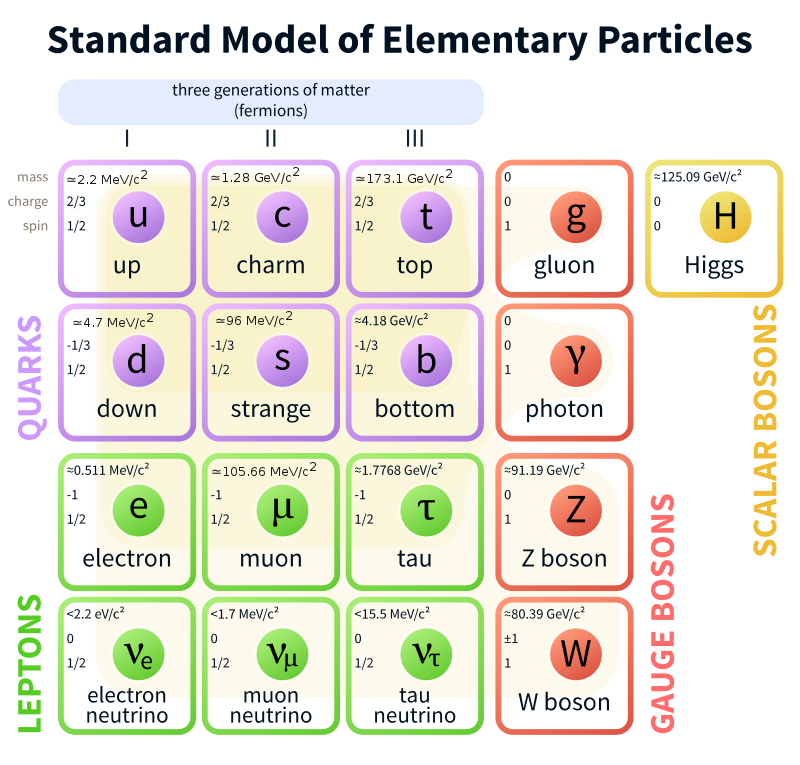
\includegraphics[width=0.7\textwidth] {Pictures/SMparticles.png}\hspace{1cm}
    \caption{Three generations of quarks and leptons are shown along with all SM bosons \cite{PDG}}
    \label{fig:SMparticles}
\end{figure}
Photons are massless, spin-1 particles and mediate all electromagnetic interactions. They couple directly to any particle with electric charge- so quarks, leptons, and $W$/$Z$ bosons but not neutrinos. Since the photon is massless, the electromagnetic force can operate on infinitely long scales but it's force decreases with $1/r^2.$
 
Gluons are massless particles with no charge and a spin-1. They couple to color charges, which are a property of quarks. Each quark has one of three colors (RGB) while anti-quarks have "anti" versions of these. Colors ore conserved 'charges' just like electric charge. Quarks are never found alone as they couple so strongly to one another as to be confined in groups of two or three. These groups are "color-confined" meaning the quarks contain colors which add up to a color neutral sum. For instance, a two quark meson $u\bar{u}$ may have colors R and anti-R while a three quark hadron $uud$ (proton) may have colors R, G, and B. Gluons are different from photons in that they are not neutral to the charge they couple to. Gluons have two colors (8 total combinations) and can thus couple to each other. This makes the strong force distinct from the electromagnetic and has implications for long-distance interactions.
 
$W$ and $Z$ bosons, unlike gluons and photons, are massive. However, like their other gauge boson counterparts, they have spin-1 and mediate a charge (weak). $W^{\pm}$ mediates charged-current interactions which can violate flavor conservation between quarks and/or leptons and their neutrinos. $Z^{0}$ mediates neutral-current interactions which conserve flavor. $W^{\pm}$ bosons contain electric charge so can interact through EM as well. In addition, $W$ and $Z$ bosons contain weak charge (as do all fermions) so can self-couple as well as couple with all fermions. 
 
The Higgs boson will be further motivated and described in later sections but suffice to say it's a massive spin-0 particle which couples to all particles with mass (including itself). It doesn't mediate any force but is still an integral part of the SM.  

\subsection{Gauge Invariance}
Quantum electrodynamics, quantum chromodynamics and the unified electro-weak theory are all examples of gauge theories, which simply means they have guage invariance symmetries. 

\subsection{Electroweak Unification}
\subsection{Spontaneous symmetry breaking}
\section{History of SM tests}
\section{LHC Physics/Phenomenology}
\section{Measurement motivation}
